\documentclass[11pt]{article}
\usepackage[margin=1in]{geometry}
\usepackage[T1]{fontenc}
\usepackage[utf8]{inputenc}
\usepackage{lmodern}
\usepackage{microtype}
\usepackage{amsmath,amssymb,mathtools}
\usepackage{booktabs}
\usepackage{graphicx}
\usepackage{xcolor}
\usepackage{hyperref}
\usepackage{enumitem}
\usepackage{tabularx}
\usepackage{float}
\usepackage{caption}
\usepackage{subcaption}

\hypersetup{
    colorlinks=true,
    linkcolor=blue!50!black,
    urlcolor=blue!60!black,
    citecolor=blue!50!black
}

% ── Notation shortcuts ──
\newcommand{\R}{\mathbb{R}}
\newcommand{\bx}{\mathbf{x}}
\newcommand{\bX}{\mathbf{X}}
\newcommand{\bz}{\mathbf{z}}
\newcommand{\bW}{\mathbf{W}}
\newcommand{\bb}{\mathbf{b}}
\newcommand{\bh}{\mathbf{h}}
\newcommand{\bs}{\mathbf{s}}
\newcommand{\bY}{\mathbf{Y}}
\newcommand{\bP}{\mathbf{P}}
\newcommand{\bH}{\mathbf{H}}
\newcommand{\bS}{\mathbf{S}}
\newcommand{\bZ}{\mathbf{Z}}
\newcommand{\bA}{\mathbf{A}}
\newcommand{\bone}{\mathbf{1}}

\title{\textbf{Math4AI Capstone: Comparative Analysis of\\Linear and Non-Linear Classifiers on\\Synthetic and Real-World Tasks}}
\author{Sharaf Feyzullayev \and Nicat Samadov \and Samir Abdullazade}
\date{\today}

\begin{document}
\maketitle

% ================================================================
%  ABSTRACT
% ================================================================
\begin{abstract}
When does a one-hidden-layer nonlinear classifier genuinely improve on a linear decision rule?
This report answers that question by comparing Softmax Regression with a single-hidden-layer
neural network ($\tanh$ activation, $H{=}32$) across three tasks of increasing geometric
complexity.  On the \emph{Linear Gaussian} task the linear model already achieves near-perfect
classification, confirming that adding a hidden layer is unnecessary when the Bayes-optimal
boundary is a hyperplane.  On the \emph{Moons} task, Softmax Regression fails
catastrophically while the neural network learns a curved boundary that perfectly separates the
two interlocking arcs.  On the \emph{Digits} benchmark ($d{=}64$, $K{=}10$) with five-seed
repeated evaluation, Softmax Regression attains $93.26\%\;\pm\;0.73\%$ test accuracy versus
$95.71\%\;\pm\;0.91\%$ for the neural network.  A Track~A PCA/SVD analysis shows that the top
20 principal components capture $89.6\%$ of variance and sustain $94.1\%$ Softmax accuracy,
revealing substantial linear structure in the input space.  A systematic failure-case study of an
$H{=}2$ bottleneck network on Digits ($58.97\%$ accuracy) demonstrates that optimisation cannot
compensate for insufficient representational capacity.  All results, derivations, and
experimental numbers reported below are produced entirely from our own NumPy implementation.
\end{abstract}

% ================================================================
%  NOTATION TABLE
% ================================================================
\vspace{-0.3em}
\noindent\textbf{Notation.}\;
We adopt the following conventions throughout.
Lowercase bold ($\bx$) denotes column vectors; uppercase bold ($\bX$) denotes matrices.
A batch of $n$ inputs is stored row-wise in $\bX\in\R^{n\times d}$.
\begin{center}
\small
\begin{tabular}{@{}ll@{\qquad}ll@{}}
\toprule
$\bx\in\R^{d}$ & input feature vector &
$\bW_1\!\in\!\R^{d\times H}$ & hidden-layer weights \\
$y\in\{1,\dots,K\}$ & true class label &
$\bW_2\!\in\!\R^{H\times K}$ & output-layer weights \\
$K$ & number of classes &
$\bb_1\!\in\!\R^{H},\;\bb_2\!\in\!\R^{K}$ & bias vectors \\
$H$ & hidden-layer width &
$\bZ^{(1)},\bZ^{(2)}$ & pre-activation matrices \\
$n$ & batch/sample size &
$\bA^{(1)}$ & hidden activations \\
$d$ & input dimension &
$\hat{\bY}\!=\!\bP$ & predicted probability matrix \\
\bottomrule
\end{tabular}
\end{center}

% ================================================================
\section{Introduction}
% ================================================================

The central question of this capstone is:
\begin{quote}
\itshape When does a one-hidden-layer nonlinear classifier genuinely improve on a linear
decision rule, and when is additional model complexity unnecessary?
\end{quote}

This is not a question that can be answered by default preference for ``deeper is better.''
A responsible comparison requires (i)~deriving the mathematics that each model class relies on,
(ii)~constructing experiments whose geometry isolates the difference, and
(iii)~evaluating with repeated seeds and honest statistics.

We study two model classes:
\begin{enumerate}[label=(\roman*),leftmargin=2em,itemsep=0.15em]
  \item \textbf{Softmax Regression}---an affine map followed by the softmax function, producing
        a linear (hyperplane) decision boundary.
  \item \textbf{One-Hidden-Layer Neural Network}---one affine map, a $\tanh$ nonlinearity, and a
        second affine map followed by softmax, producing a nonlinear decision boundary whose
        shape depends on the hidden width~$H$.
\end{enumerate}

Both models are evaluated on three tasks chosen to span a spectrum of geometric difficulty:
\begin{itemize}[leftmargin=1.4em,itemsep=0.15em]
  \item \textbf{Linear Gaussian}: two isotropic Gaussian blobs in $\R^2$---linearly separable by
        construction.
  \item \textbf{Moons}: two interleaving half-circles in $\R^2$---not separable by any
        hyperplane.
  \item \textbf{Digits}: an $8{\times}8$ handwritten-digit dataset ($d{=}64$, $K{=}10$) with a
        fixed train/validation/test split.
\end{itemize}

Every model and optimiser is implemented from scratch in NumPy; no automatic-differentiation
libraries are used.

% ================================================================
\section{Background and Mathematical Setup}
% ================================================================

\subsection{Softmax Cross-Entropy as Negative Log-Likelihood}

Consider a probabilistic classifier that, for each input $\bx\in\R^d$, parameterises a
categorical distribution over $K$ classes via logits $\bz = \bW\bx + \bb$, where
$\bW\in\R^{K\times d}$ and $\bb\in\R^K$.  The softmax function converts logits to probabilities:
\begin{equation}\label{eq:softmax}
  \hat{y}_k \;=\; P(y{=}k\mid\bx)
  \;=\; \frac{\exp(z_k)}{\displaystyle\sum_{j=1}^{K}\exp(z_j)},
  \qquad k=1,\dots,K.
\end{equation}

\paragraph{Derivation of the NLL.}
Given $N$ independent training pairs $\{(\bx^{(i)},y^{(i)})\}_{i=1}^{N}$, the likelihood of the
observed labels under the model is
\[
  \mathcal{L}(\bW,\bb)
  \;=\;\prod_{i=1}^{N} P\!\bigl(y^{(i)}\mid\bx^{(i)}\bigr)
  \;=\;\prod_{i=1}^{N} \hat{y}_{y^{(i)}}^{(i)}.
\]
Taking the logarithm converts products to sums and avoids numerical underflow:
\[
  \log\mathcal{L}
  \;=\;\sum_{i=1}^{N} \log \hat{y}_{y^{(i)}}^{(i)}.
\]
With one-hot labels $\mathbf{y}^{(i)}\in\{0,1\}^K$ (i.e.\ $y^{(i)}_k=1$ iff $k$ is the true
class), this can be rewritten as
$\sum_{i}\sum_{k} y^{(i)}_k \log \hat{y}^{(i)}_k$,
since only the $k{=}y^{(i)}$ term survives.
Negating and averaging over the dataset yields the cross-entropy loss:
\begin{equation}\label{eq:ce}
  J \;=\; -\,\frac{1}{N}\sum_{i=1}^{N}\sum_{k=1}^{K} y_k^{(i)}\log\hat{y}_k^{(i)}.
\end{equation}
Therefore, \textbf{minimising cross-entropy is algebraically identical to maximising the
log-likelihood} of the observed labels under the categorical model~\eqref{eq:softmax}.
This is not a heuristic choice: the loss function is the direct consequence of treating
classification as probabilistic inference.

\paragraph{Connection to regularisation.}
Adding an $L_2$ penalty $\frac{\lambda}{2}\|\bW\|_F^2$ to $J$ is equivalent to placing an
isotropic Gaussian prior $\bW\sim\mathcal{N}(\mathbf{0},\lambda^{-1}\mathbf{I})$ and performing
maximum-a-posteriori (MAP) estimation rather than pure MLE.  We use $\lambda=10^{-4}$ throughout.

% ──────────────────────────────────────────────────────────────────
\subsection{Conceptual Overview of Backpropagation}
\label{sec:backprop-concept}

Before writing any gradient formulas, it is important to understand what backpropagation
\emph{does}, not just \emph{how} it computes.

In the forward pass, data flows from the input~$\bx$ through a sequence of parameterised
transformations---affine projections, element-wise nonlinearities, softmax---to produce a scalar
loss~$J$.  Each intermediate quantity (pre-activations, hidden activations, logits, probabilities)
is saved.

Backpropagation is the systematic, reverse-order application of the multivariate chain rule
through this computation graph.  Starting from the output, we compute how the loss changes with
respect to the predicted probabilities.  We then step backward, layer by layer: at each stage, we
multiply the incoming ``error signal'' (the gradient from the layer above) by the local Jacobian
of the current transformation.  This decomposes the global objective into \emph{localised}
directional updates for every individual weight.

Concretely, backpropagation answers the question:
\begin{quote}
\itshape If the loss changed by a small amount, which parameters are responsible, in which
direction, and by how much?
\end{quote}

The beauty of the procedure is that each local derivative is simple---a matrix transpose, an
element-wise activation derivative, a sum---and the chain rule assembles them into exact
parameter gradients at a cost proportional to one extra forward pass.  No finite differences or
approximations are involved.

% ──────────────────────────────────────────────────────────────────
\subsection{Complete Gradient Derivation for the One-Hidden-Layer Network}
\label{sec:gradient-derivation}

We now derive the parameter gradients in full.
Consider a minibatch $\bX\in\R^{n\times d}$ with one-hot label matrix $\bY\in\{0,1\}^{n\times K}$.

\paragraph{Forward pass.}
The computation proceeds in four stages:
\begin{align}
  \bZ^{(1)} &= \bX\,\bW_1 + \bone\,\bb_1^\top
    & &\in\R^{n\times H}, \label{eq:fwd1}\\
  \bA^{(1)} &= \tanh\!\bigl(\bZ^{(1)}\bigr)
    & &\in\R^{n\times H}, \label{eq:fwd2}\\
  \bZ^{(2)} &= \bA^{(1)}\bW_2 + \bone\,\bb_2^\top
    & &\in\R^{n\times K}, \label{eq:fwd3}\\
  \hat{\bY}  &= \mathrm{softmax}_{\text{row}}\!\bigl(\bZ^{(2)}\bigr)
    & &\in\R^{n\times K}. \label{eq:fwd4}
\end{align}

\paragraph{Loss.}
The average cross-entropy over the minibatch is
\begin{equation}\label{eq:batch-ce}
  J = -\frac{1}{n}\sum_{i=1}^{n}\sum_{k=1}^{K} Y_{ik}\log\hat{Y}_{ik}.
\end{equation}

\paragraph{Step 1: Output-layer error.}
A classical result from the calculus of softmax combined with cross-entropy shows that the
gradient with respect to the output logits simplifies to the prediction residual:
\begin{equation}\label{eq:delta2}
  \boldsymbol{\delta}^{(2)}
  \;=\;\frac{\partial J}{\partial \bZ^{(2)}}
  \;=\;\frac{1}{n}\bigl(\hat{\bY}-\bY\bigr).
\end{equation}
\emph{Derivation sketch:} For each sample $i$ and class $k$,
$\frac{\partial J}{\partial Z^{(2)}_{ik}}
= -\frac{1}{n}\bigl(\sum_j Y_{ij}\,\frac{\partial\log\hat{Y}_{ij}}{\partial Z^{(2)}_{ik}}\bigr)
= \frac{1}{n}(\hat{Y}_{ik}-Y_{ik})$,
using $\frac{\partial\log\hat{Y}_{ij}}{\partial Z^{(2)}_{ik}}=\delta_{jk}-\hat{Y}_{ik}$.

\paragraph{Step 2: Output-layer parameter gradients.}
Since $\bZ^{(2)}=\bA^{(1)}\bW_2+\bone\bb_2^\top$:
\begin{align}
  \frac{\partial J}{\partial \bW_2}
  &= \bigl(\bA^{(1)}\bigr)^\top \boldsymbol{\delta}^{(2)}
  \;\in\;\R^{H\times K},
  \label{eq:gW2}\\[4pt]
  \frac{\partial J}{\partial \bb_2}
  &= \bigl(\boldsymbol{\delta}^{(2)}\bigr)^\top\bone
  \;\in\;\R^{K}.
  \label{eq:gb2}
\end{align}

\paragraph{Step 3: Hidden-layer error (back-propagation through $\tanh$).}
We transport the error through the second linear map and modulate by the local
$\tanh$ derivative, $\tanh'(z)=1-\tanh^2(z)$:
\begin{equation}\label{eq:delta1}
  \boldsymbol{\delta}^{(1)}
  \;=\;
  \bigl(\boldsymbol{\delta}^{(2)}\,\bW_2^\top\bigr)
  \;\odot\;
  \bigl(1-\bA^{(1)}\odot\bA^{(1)}\bigr),
  \qquad\in\R^{n\times H}.
\end{equation}
Here $\odot$ denotes the Hadamard (element-wise) product.  The first factor propagates the error
across the linear boundary $\bW_2$; the second factor scales each component by how responsive the
$\tanh$ activation is at that point.

\paragraph{Step 4: Hidden-layer parameter gradients.}
Since $\bZ^{(1)}=\bX\bW_1+\bone\bb_1^\top$:
\begin{align}
  \frac{\partial J}{\partial \bW_1}
  &= \bX^\top\,\boldsymbol{\delta}^{(1)}
  \;\in\;\R^{d\times H},
  \label{eq:gW1}\\[4pt]
  \frac{\partial J}{\partial \bb_1}
  &= \bigl(\boldsymbol{\delta}^{(1)}\bigr)^\top\bone
  \;\in\;\R^{H}.
  \label{eq:gb1}
\end{align}

These four steps constitute the complete backpropagation for our architecture.
When $L_2$ regularisation is used, we additionally add $\lambda\bW_\ell$ to each weight gradient.

% ──────────────────────────────────────────────────────────────────
\subsection{Geometric Compatibility: Gaussian vs.\ Moons}
\label{sec:geometry}

\paragraph{Why the Gaussian task matches a linear decision rule.}
The Linear Gaussian dataset consists of two classes drawn from multivariate normals with distinct
means $\boldsymbol{\mu}_0,\boldsymbol{\mu}_1\in\R^2$ and a shared isotropic covariance
$\Sigma=\sigma^2\mathbf{I}$.  The log-odds between the two classes is
\[
  \log\frac{P(y{=}1\mid\bx)}{P(y{=}0\mid\bx)}
  \;=\;
  \frac{1}{\sigma^2}\bigl(\boldsymbol{\mu}_1-\boldsymbol{\mu}_0\bigr)^\top\bx
  \;+\;\text{const},
\]
which is an \emph{affine} function of~$\bx$.  Hence the Bayes-optimal decision boundary is a
straight line (hyperplane in general), and Softmax Regression can exactly represent it.  A hidden
layer adds parameters but cannot change the boundary geometry in a meaningful way.

\paragraph{Why the Moons task requires nonlinearity.}
The Moons dataset arranges two classes in interleaving half-circles whose supports curve into each
other's coordinate space.  No single hyperplane can separate the two arcs without extensive
misclassification.  The decision boundary must \emph{curve}, which requires a nonlinear
transformation of the input coordinates.  The hidden layer's role (Section~\ref{sec:discussion})
is to learn such a transformation: mapped into $\R^H$ via $\tanh(\bW_1\bx+\bb_1)$, the
previously entangled points become linearly separable, after which the second affine map can draw
a hyperplane in the new space.

% ================================================================
\section{Methods}
% ================================================================

\paragraph{Datasets.}
Three datasets are used, all loaded from the starter pack:
\begin{enumerate}[label=\arabic*.,leftmargin=2em,itemsep=0.15em]
  \item \textbf{Linear Gaussian}: 400 points in $\R^2$, two linearly separable blobs.
  \item \textbf{Moons}: 400 points in $\R^2$, two interlocking half-circles.
  \item \textbf{Digits}: $d{=}64$ pixel features from the UCI handwritten digits dataset,
        stratified into 1\,258~train / 270~validation / 269~test samples, $K{=}10$ classes.
\end{enumerate}

\paragraph{Implementation.}
Both models are implemented entirely in NumPy with no automatic differentiation.  Softmax is
computed in a numerically stable manner by subtracting the row-wise maximum before
exponentiation.  Gradients follow the derivations in Section~\ref{sec:gradient-derivation}.

\paragraph{Training protocol.}
For the Digits benchmark a strict protocol is followed:
\begin{itemize}[leftmargin=1.4em,itemsep=0.15em]
  \item Mini-batch size: $64$.
  \item $L_2$ regularisation: $\lambda=10^{-4}$ for both models.
  \item Epoch budget: 200.
  \item Model selection: checkpoint with the lowest \emph{validation} cross-entropy
        is retained as the final model.
  \item Softmax baseline optimiser: mini-batch SGD, learning rate $0.05$.
  \item Neural-network default: hidden width $H{=}32$, SGD with learning rate $0.05$.
\end{itemize}

For the two synthetic tasks, both models are trained with full-batch gradient descent for a fixed
number of epochs (1\,000 for Gaussian, 2\,000 for Moons) and the final epoch is reported.

\paragraph{Repeated-seed evaluation.}
On the Digits benchmark, each final configuration (Softmax and Neural Network) is run with five
random seeds.  For each seed the test set is evaluated \emph{exactly once} after selecting the
best validation checkpoint.  We report mean accuracy, mean cross-entropy, and a $95\%$ confidence
interval
\(
  \bar{x}\pm t_{0.025,4}\cdot s/\!\sqrt{5}
  = \bar{x}\pm 2.776\cdot s/\!\sqrt{5}
\),
where $s$ is the sample standard deviation.

% ================================================================
\section{Implementation Sanity Checks}
% ================================================================

Before running any experiment, three automated checks (\texttt{sanity\_checks.py}) verified
fundamental correctness:

\begin{enumerate}[label=\textbf{Check~\arabic*.},leftmargin=3em,itemsep=0.3em]
  \item \textbf{Probability normalisation.}
        On three test logit vectors (including the extreme case
        $\bz=[-100,\;0,\;100]$), the \texttt{stable\_softmax} function returns rows that sum to
        $1.0$ to machine precision.
        \hfill$\checkmark$\;PASS

  \item \textbf{Overfitting a micro-dataset.}
        A neural network with $H{=}16$ was trained on 5~hand-chosen $2$-D samples for 150~Adam
        steps.  The final loss fell below $0.05$ and classification accuracy reached $100\%$,
        confirming that forward and backward passes are mutually consistent.
        \hfill$\checkmark$\;PASS

  \item \textbf{Monotonic loss decrease.}
        A fresh Softmax Regression model with random parameters was updated for 10 SGD steps on a
        50-sample batch (4 features, 3 classes, no regularisation).  The loss decreased
        monotonically from $1.1282$ to $0.9357$, indicating correct gradient direction.
        \hfill$\checkmark$\;PASS
\end{enumerate}

All three checks pass automatically; no NaN or Inf values were encountered during any experiment.

% ================================================================
\section{Experiments}
% ================================================================

\subsection{Synthetic Decision Boundaries}

\paragraph{Linear Gaussian.}
Figure~\ref{fig:comparison_gaussian} shows that both models learn essentially the same straight
boundary.  The neural network adds curvature to the probability contours but does not change the
location of the $50\%$-probability line.  Both achieve near-perfect accuracy, confirming the
geometric argument of Section~\ref{sec:geometry}: when the Bayes-optimal boundary is a
hyperplane, the hidden layer provides no representational advantage.

\begin{figure}[H]
  \centering
  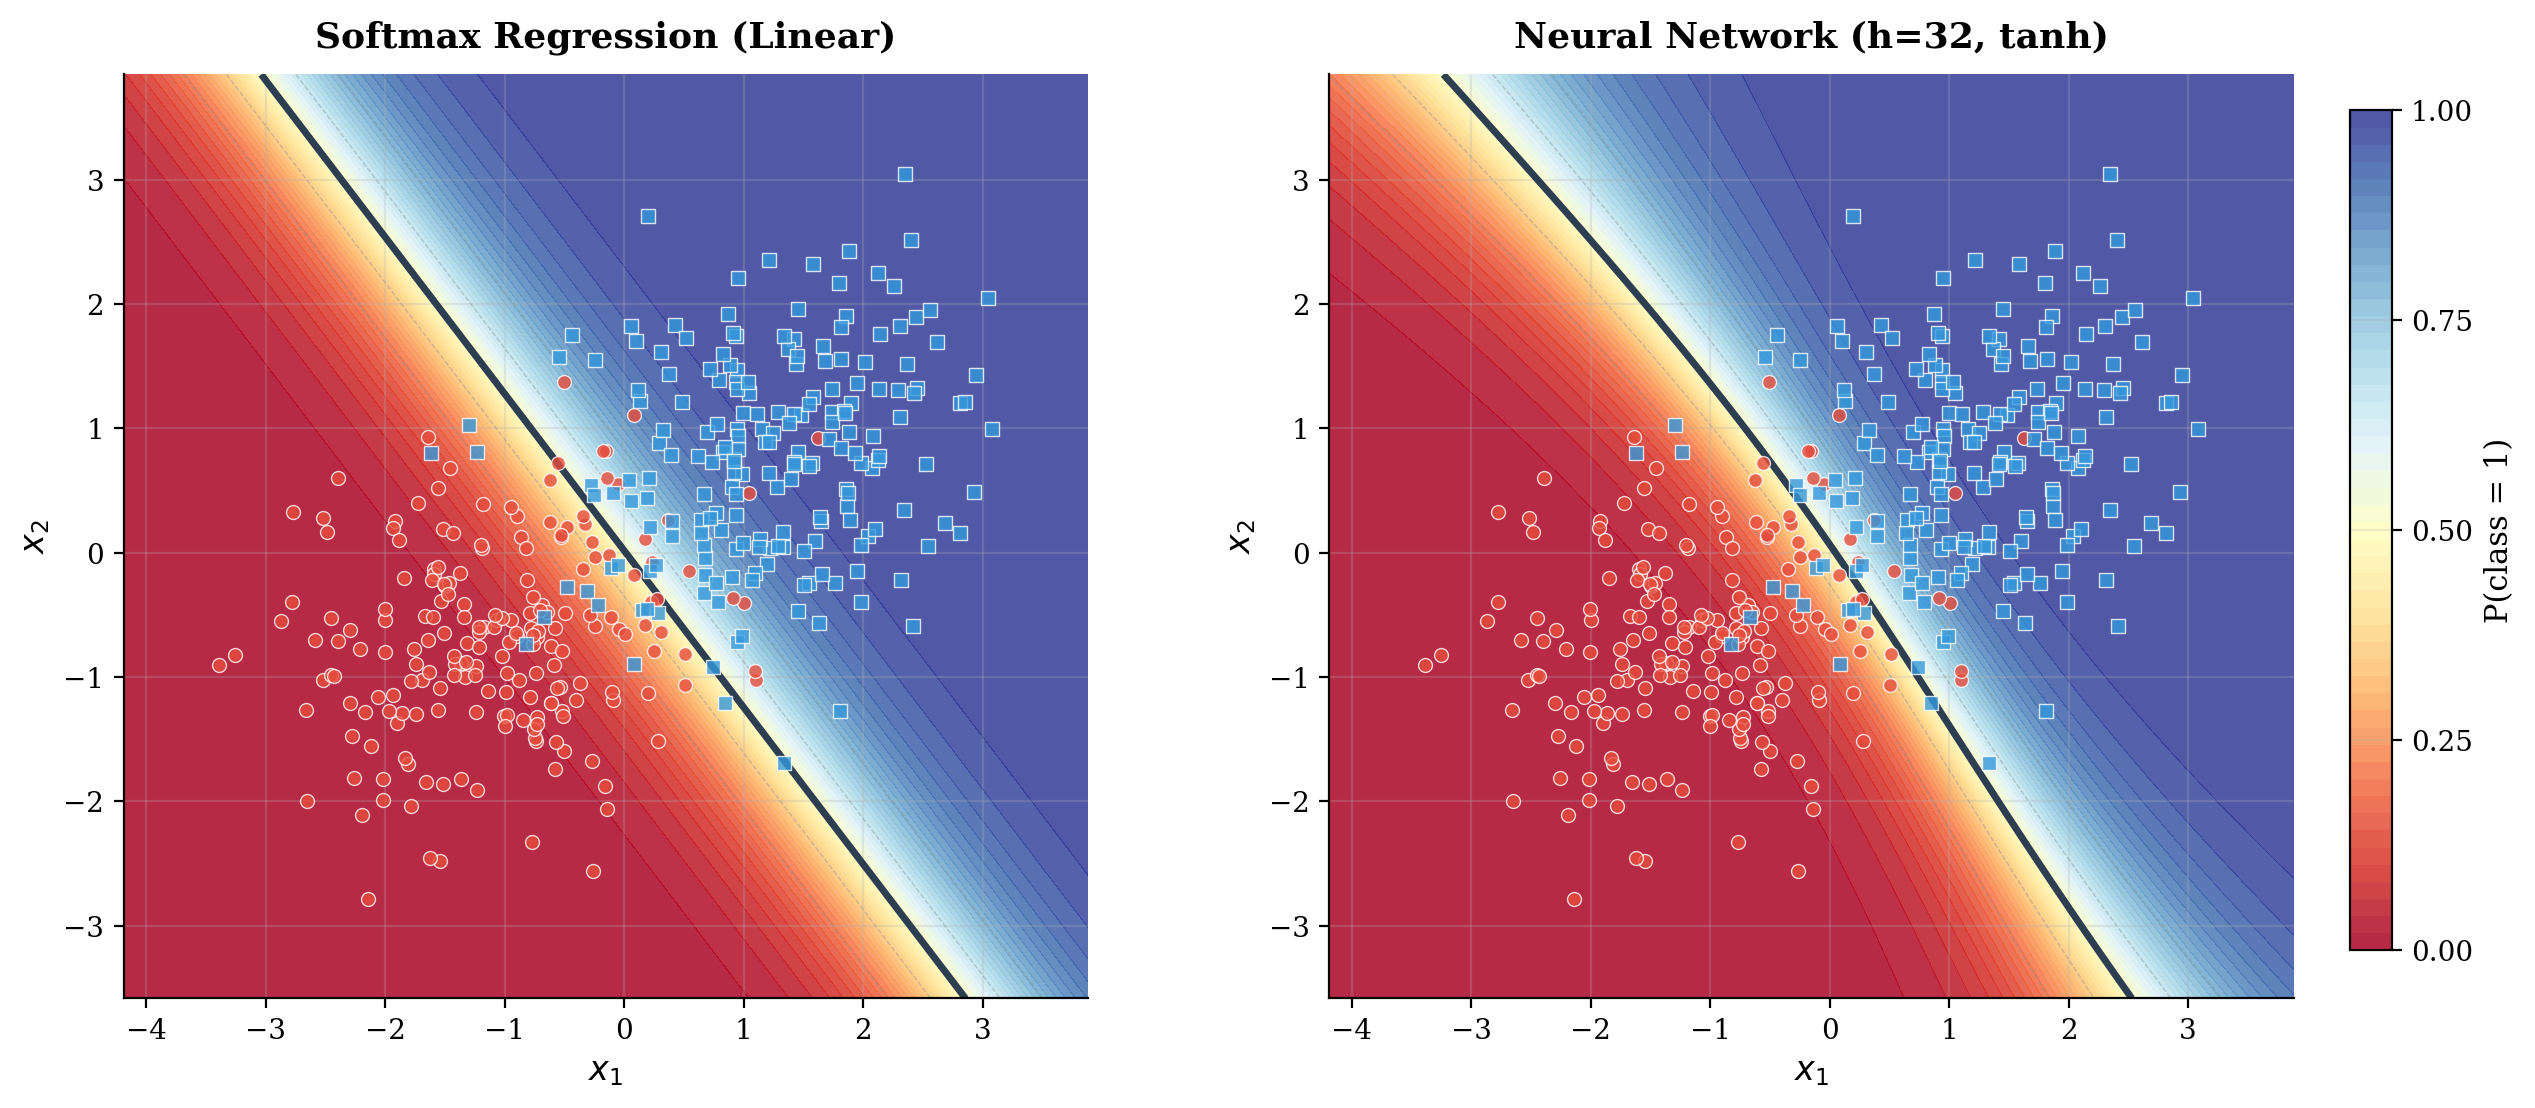
\includegraphics[width=\textwidth]{../figures/comparison_lineargaussian.png}
  \caption{Decision boundaries on the Linear Gaussian task.  Left: Softmax Regression.
           Right: Neural Network ($H{=}32$).  Both produce a near-identical linear separator.}
  \label{fig:comparison_gaussian}
\end{figure}

\paragraph{Moons.}
Figure~\ref{fig:comparison_moons} highlights the fundamental geometric difference.
Softmax Regression is forced to place a straight line through the curved data, resulting in
substantial misclassification.  The neural network ($H{=}32$) warps the input space via $\tanh$
and draws a smooth, curved boundary that separates the two arcs with near-$100\%$ accuracy.

\begin{figure}[H]
  \centering
  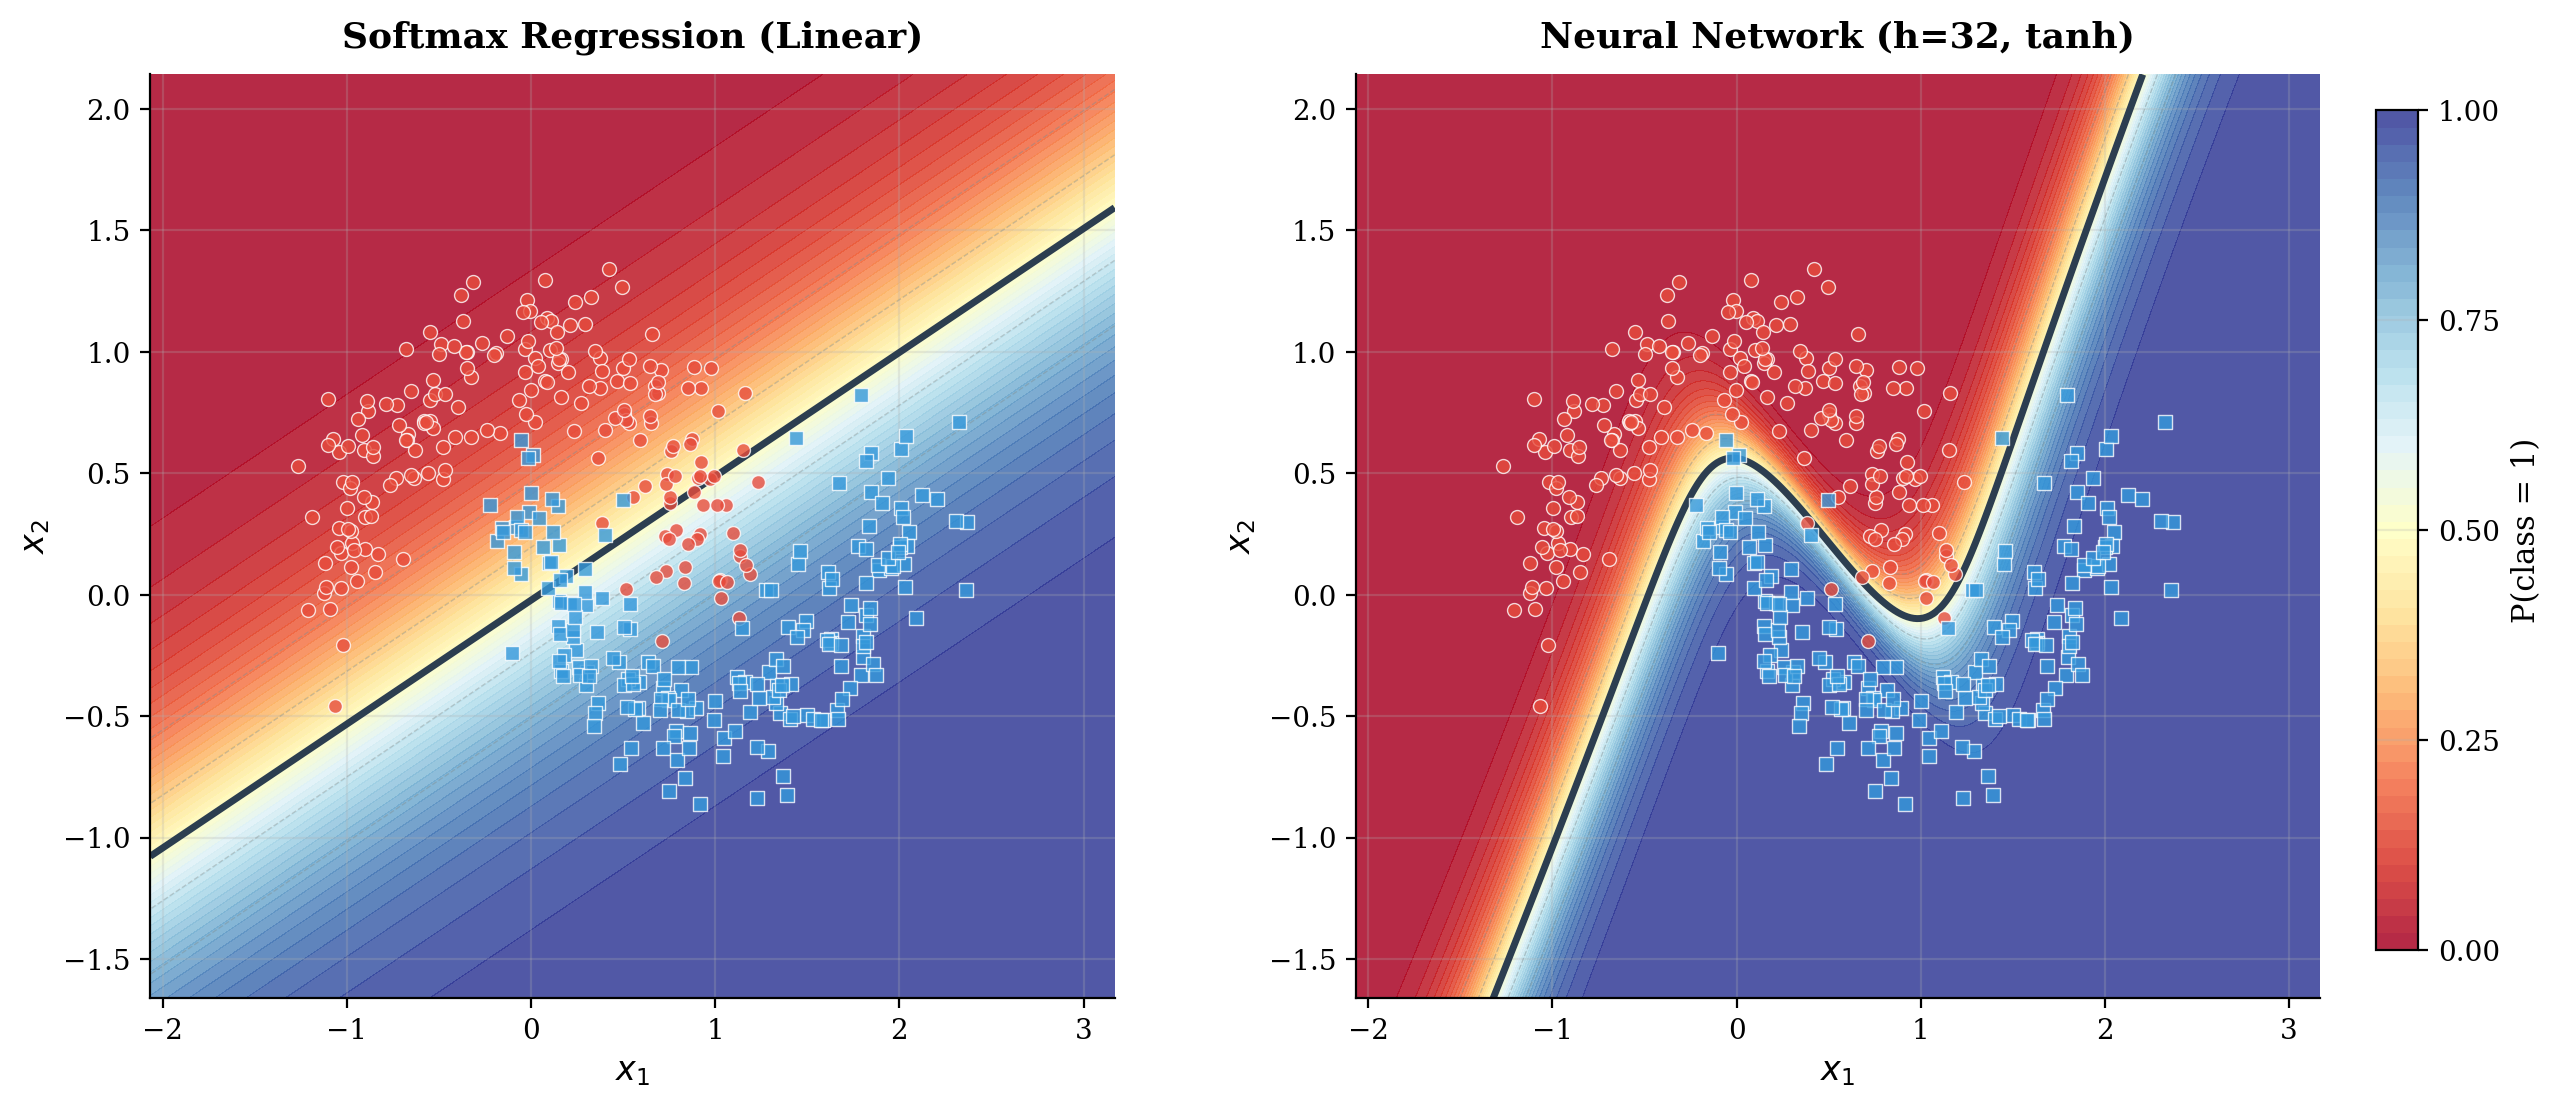
\includegraphics[width=\textwidth]{../figures/comparison_moons.png}
  \caption{Decision boundaries on the Moons task.  Left: Softmax Regression (linear, fails).
           Right: Neural Network ($H{=}32$, succeeds).}
  \label{fig:comparison_moons}
\end{figure}

% ──────────────────────────────────────────────────────────────────
\subsection{Capacity Ablation on Moons}

We trained the neural network on the Moons task with hidden widths $H\in\{2,8,32\}$
(Figure~\ref{fig:ablation}).

\begin{itemize}[leftmargin=1.4em,itemsep=0.15em]
  \item $H{=}2$: Only two hidden units are available to span the transformed space.  The model
        produces angular, low-confidence boundaries and fails to capture the full curvature.
  \item $H{=}8$: A reasonable approximation to the curved boundary emerges, though confidence is
        still uneven near the boundary.
  \item $H{=}32$: The boundary is smooth, high-confidence, and tightly hugs the data manifold.
\end{itemize}

This ablation demonstrates a clear monotonic relationship between hidden width and boundary
quality \emph{on this task}.  It does not, however, imply that $H{=}32$ is universally optimal;
on the Gaussian task, all three widths produce essentially the same linear boundary.

\begin{figure}[H]
  \centering
  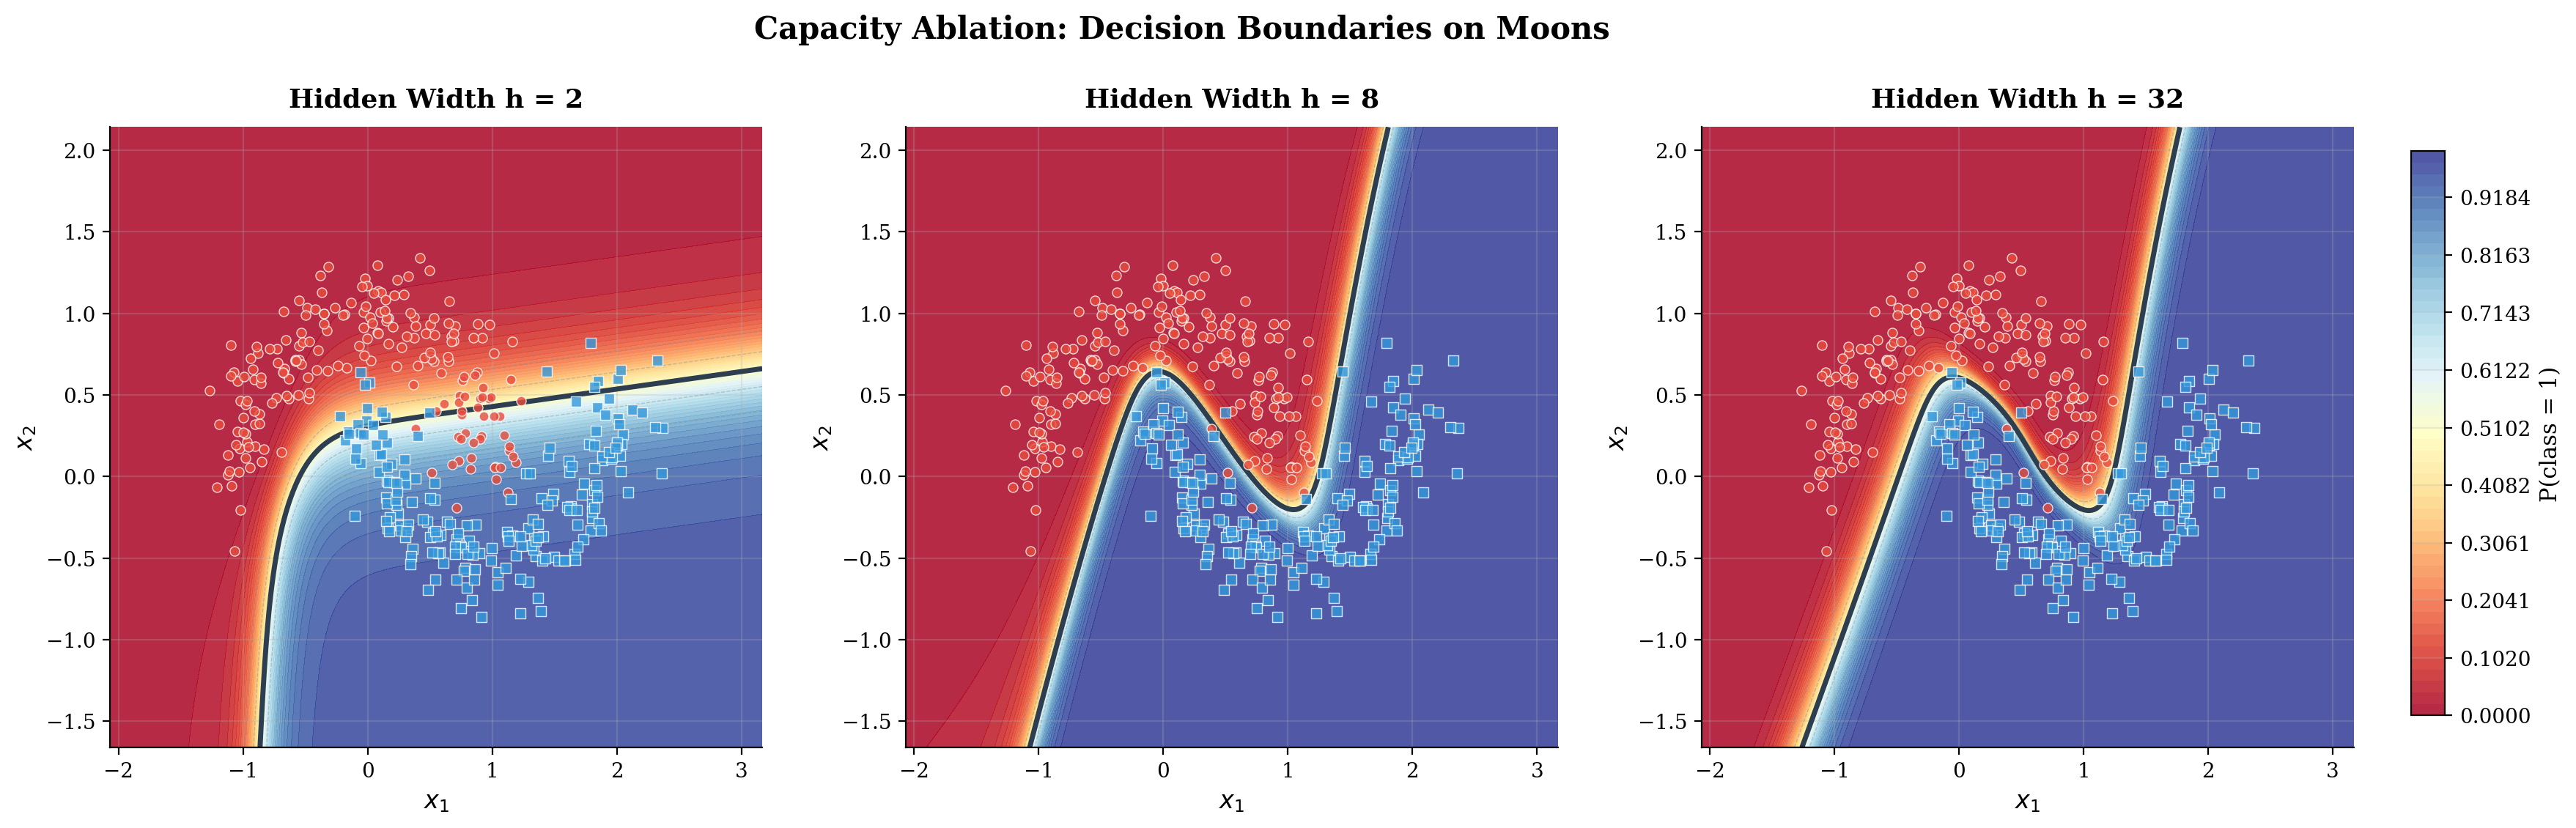
\includegraphics[width=\textwidth]{../figures/capacity_ablation_boundaries.png}
  \caption{Capacity ablation on Moons.  From left to right: $H{=}2$, $H{=}8$, $H{=}32$.
           Boundary smoothness and classification confidence increase with hidden width.}
  \label{fig:ablation}
\end{figure}

% ──────────────────────────────────────────────────────────────────
\subsection{Digits Benchmark}

Table~\ref{tab:digits_main} summarises the core Digits comparison using the validation-selected
best checkpoint over 200~epochs.

\begin{table}[H]
\centering
\caption{Digits benchmark: five-seed summary (mean $\pm$ 95\% CI).}
\label{tab:digits_main}
\begin{tabular}{@{}lcc@{}}
\toprule
\textbf{Model} & \textbf{Test Accuracy} & \textbf{Test Cross-Entropy} \\
\midrule
Softmax Regression & $93.26\%\;\pm\;0.73\%$ & $0.2692\;\pm\;0.0067$ \\
Neural Network ($H{=}32$) & $95.71\%\;\pm\;0.91\%$ & $0.1566\;\pm\;0.0162$ \\
\bottomrule
\end{tabular}
\end{table}

The neural network improves test accuracy by ${\sim}2.5$ percentage points and reduces
cross-entropy by ${\sim}42\%$.  The gain is modest but statistically consistent: the
$95\%$ confidence intervals for the two models do not overlap.
Figure~\ref{fig:loss_curves_digits} shows representative training and validation loss curves.

\begin{figure}[H]
  \centering
  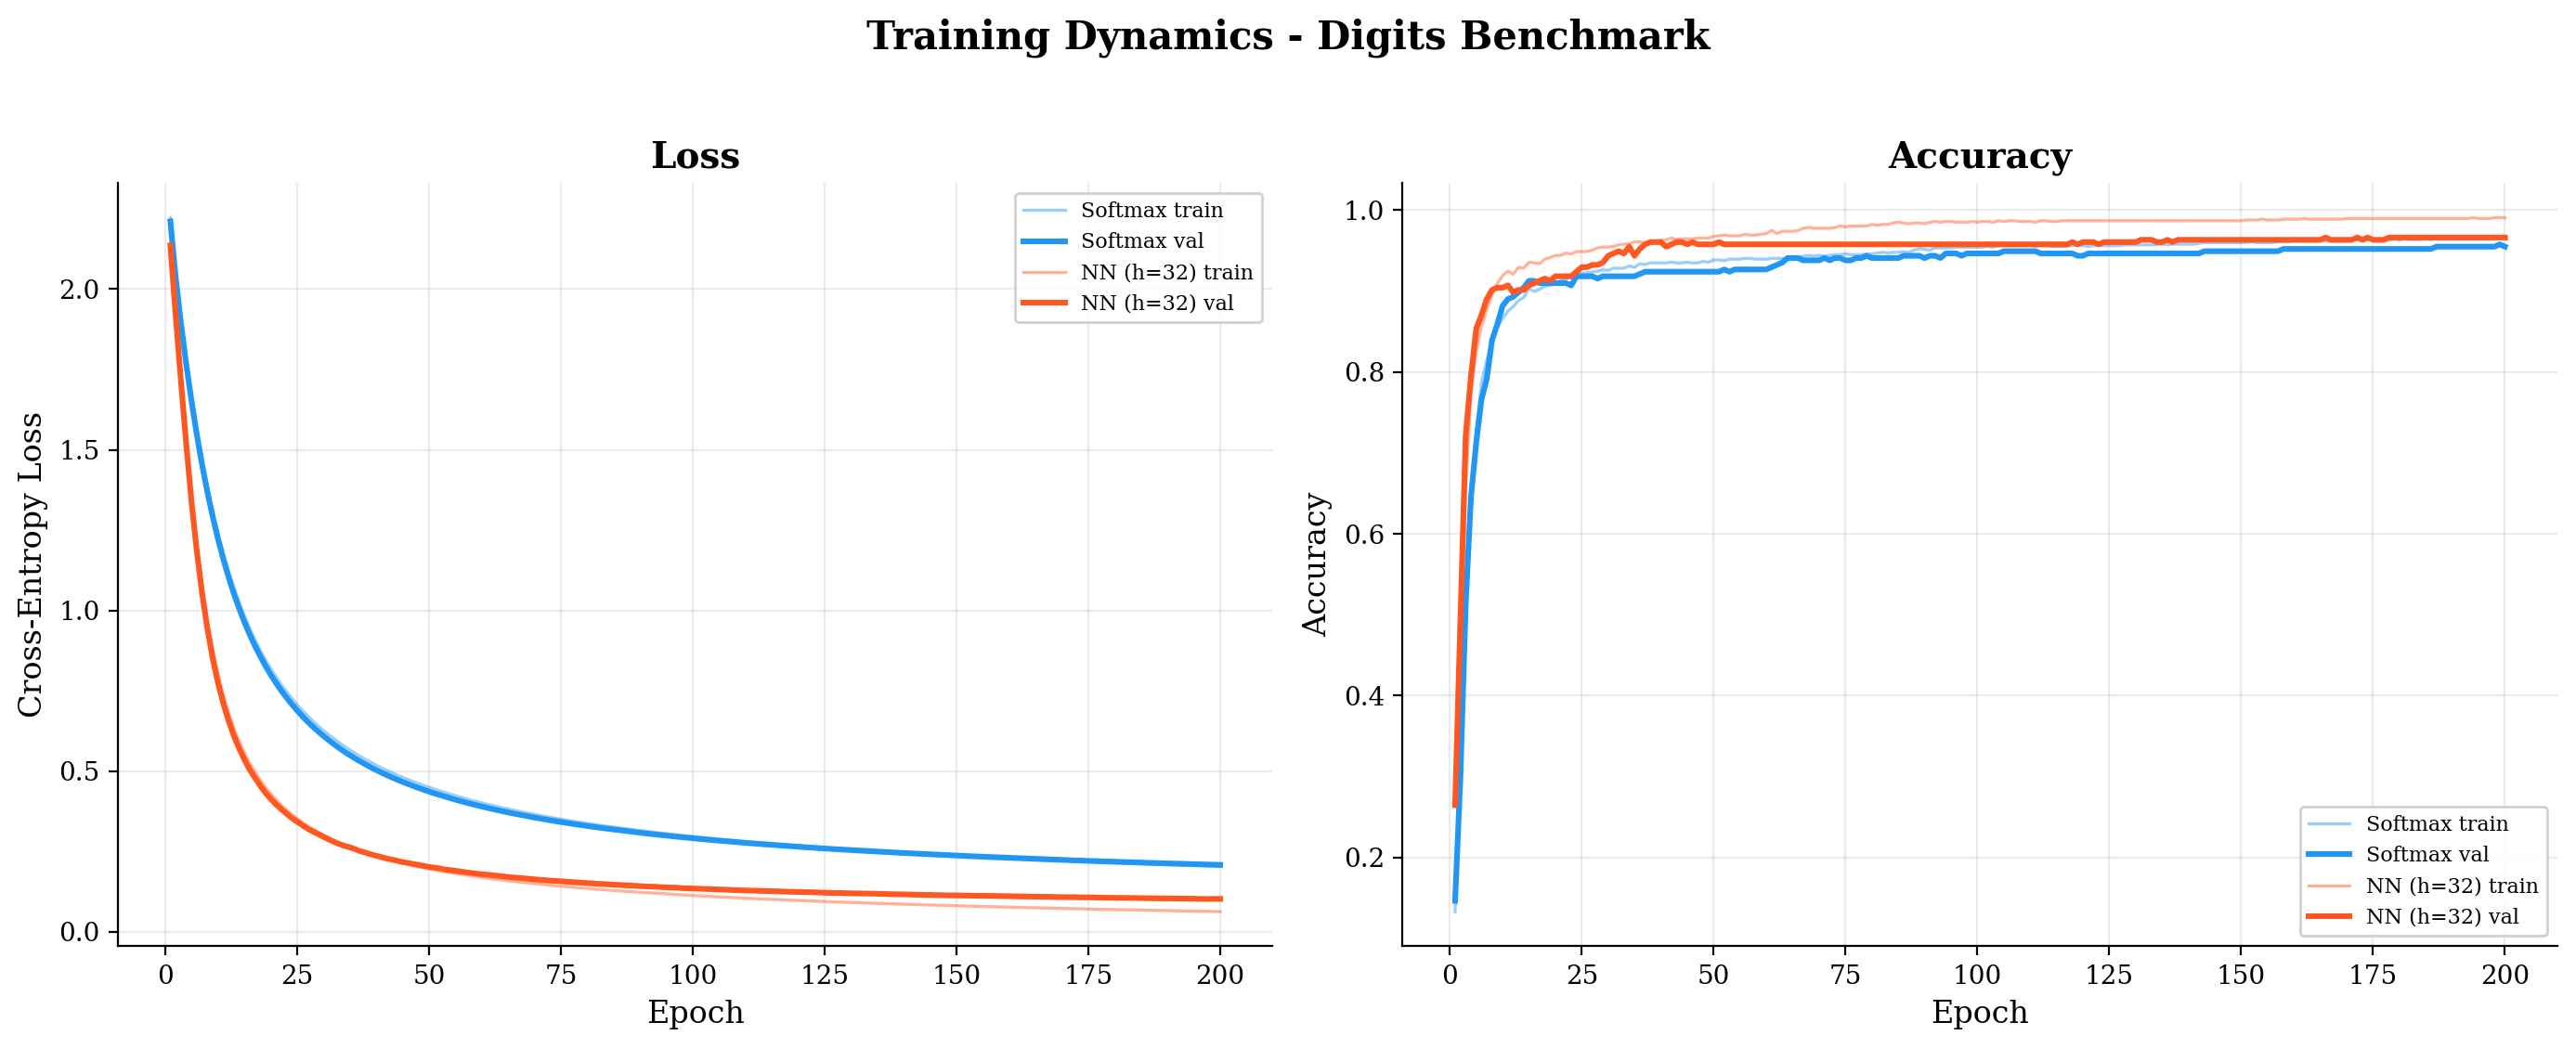
\includegraphics[width=\textwidth]{../figures/loss_curves_digits.png}
  \caption{Training dynamics on the Digits benchmark (single representative seed).}
  \label{fig:loss_curves_digits}
\end{figure}

% ──────────────────────────────────────────────────────────────────
\subsection{Optimizer Study on Digits}
\label{sec:optimizer}

Three optimisers were compared on the neural network ($H{=}32$) using fixed hyperparameters from
the Digits protocol:

\begin{table}[H]
\centering
\caption{Optimizer study on Digits (NN, $H{=}32$, best validation checkpoint).}
\label{tab:optimizers}
\begin{tabular}{@{}lccc@{}}
\toprule
\textbf{Optimizer} & \textbf{Test Acc.} & \textbf{Test CE} & \textbf{Best Epoch} \\
\midrule
SGD ($\eta{=}0.05$) & 94.84\% & 0.1700 & 197 \\
Momentum ($\eta{=}0.05,\;\mu{=}0.9$) & 95.38\% & 0.1653 & 197 \\
Adam ($\eta{=}0.001$) & 95.11\% & 0.1507 & 197 \\
\bottomrule
\end{tabular}
\end{table}

Figure~\ref{fig:optimizers} visualises the validation dynamics.  Adam and Momentum converge to
low validation loss significantly faster than plain SGD, but all three reach comparable final
accuracy within the 200-epoch budget.  Adam achieves the lowest final cross-entropy ($0.1507$),
which indicates better-calibrated probabilities even though its accuracy is slightly below
Momentum's.  The practical conclusion is that, for this small-scale task, the choice of optimiser
has a measurable but secondary effect relative to the choice of model class.

\begin{figure}[H]
  \centering
  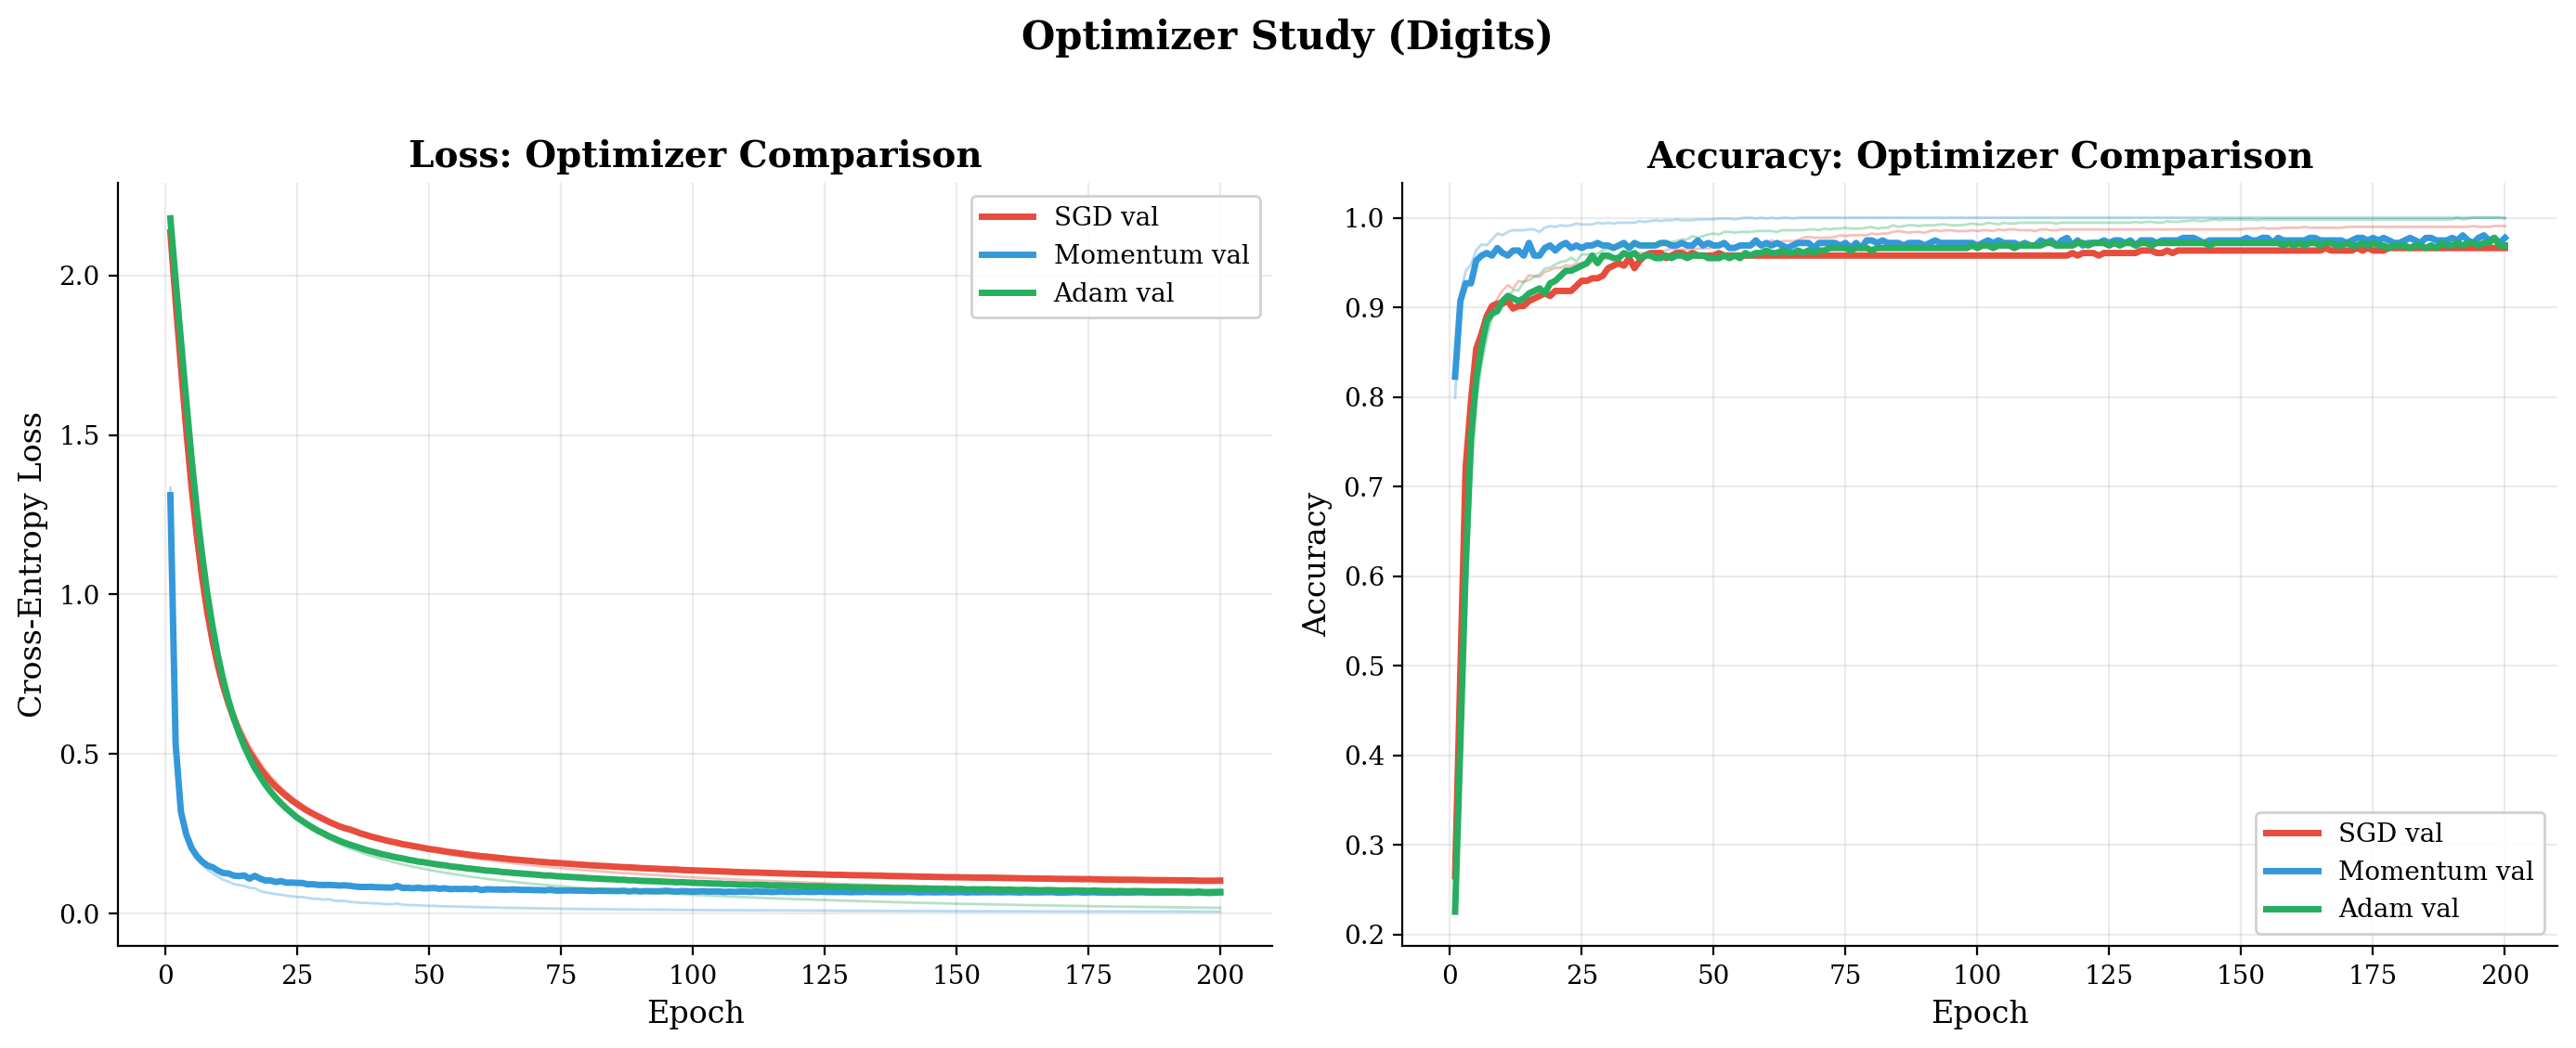
\includegraphics[width=\textwidth]{../figures/optimizer_study_digits.png}
  \caption{Validation loss and accuracy across optimisers (NN, $H{=}32$, Digits).}
  \label{fig:optimizers}
\end{figure}

% ──────────────────────────────────────────────────────────────────
\subsection{Failure-Case Analysis: Under-Capacity Bottleneck ($H{=}2$)}
\label{sec:failure}

We deliberately trained a neural network with $H{=}2$ on the 10-class Digits task.  The hidden
layer maps the 64-dimensional input to a 2-dimensional representation via
$\bh=\tanh(\bW_1\bx+\bb_1)$ before attempting to classify into 10~classes.

\begin{table}[H]
\centering
\caption{Failure case: $H{=}2$ bottleneck on Digits.}
\begin{tabular}{@{}lcc@{}}
\toprule
\textbf{Model} & \textbf{Test Accuracy} & \textbf{Test Cross-Entropy} \\
\midrule
NN ($H{=}2$) & 58.97\% & 1.1133 \\
NN ($H{=}32$) & 95.71\% & 0.1566 \\
\bottomrule
\end{tabular}
\end{table}

The $H{=}2$ model achieves only $58.97\%$ accuracy---far below even the linear baseline
($93.26\%$).  Despite using the same optimiser, learning rate, and epoch budget, the model
\emph{underfits}: both training and validation loss remain high throughout.

\paragraph{Why it fails.}
The failure is \emph{representational}, not optimisational.  With only 2 hidden units, the
network is forced to represent \emph{all} inter-class structure through a 2-dimensional
bottleneck.  The second layer then tries to cut this 2-D space into 10 regions with 10 linear
half-spaces, but two dimensions are simply insufficient to arrange 10 classes into linearly
separable clusters.  The optimiser faithfully finds the best possible mapping given the
architecture, but the best possible mapping is poor.

This demonstrates a fundamental principle: \textbf{representational capacity must match task
complexity before optimisation can be effective.}  Adding hidden units from $H{=}2$ to $H{=}32$
does not change the optimiser; it changes the \emph{geometry of the function class}, enabling
richer internal representations.

\begin{figure}[H]
  \centering
  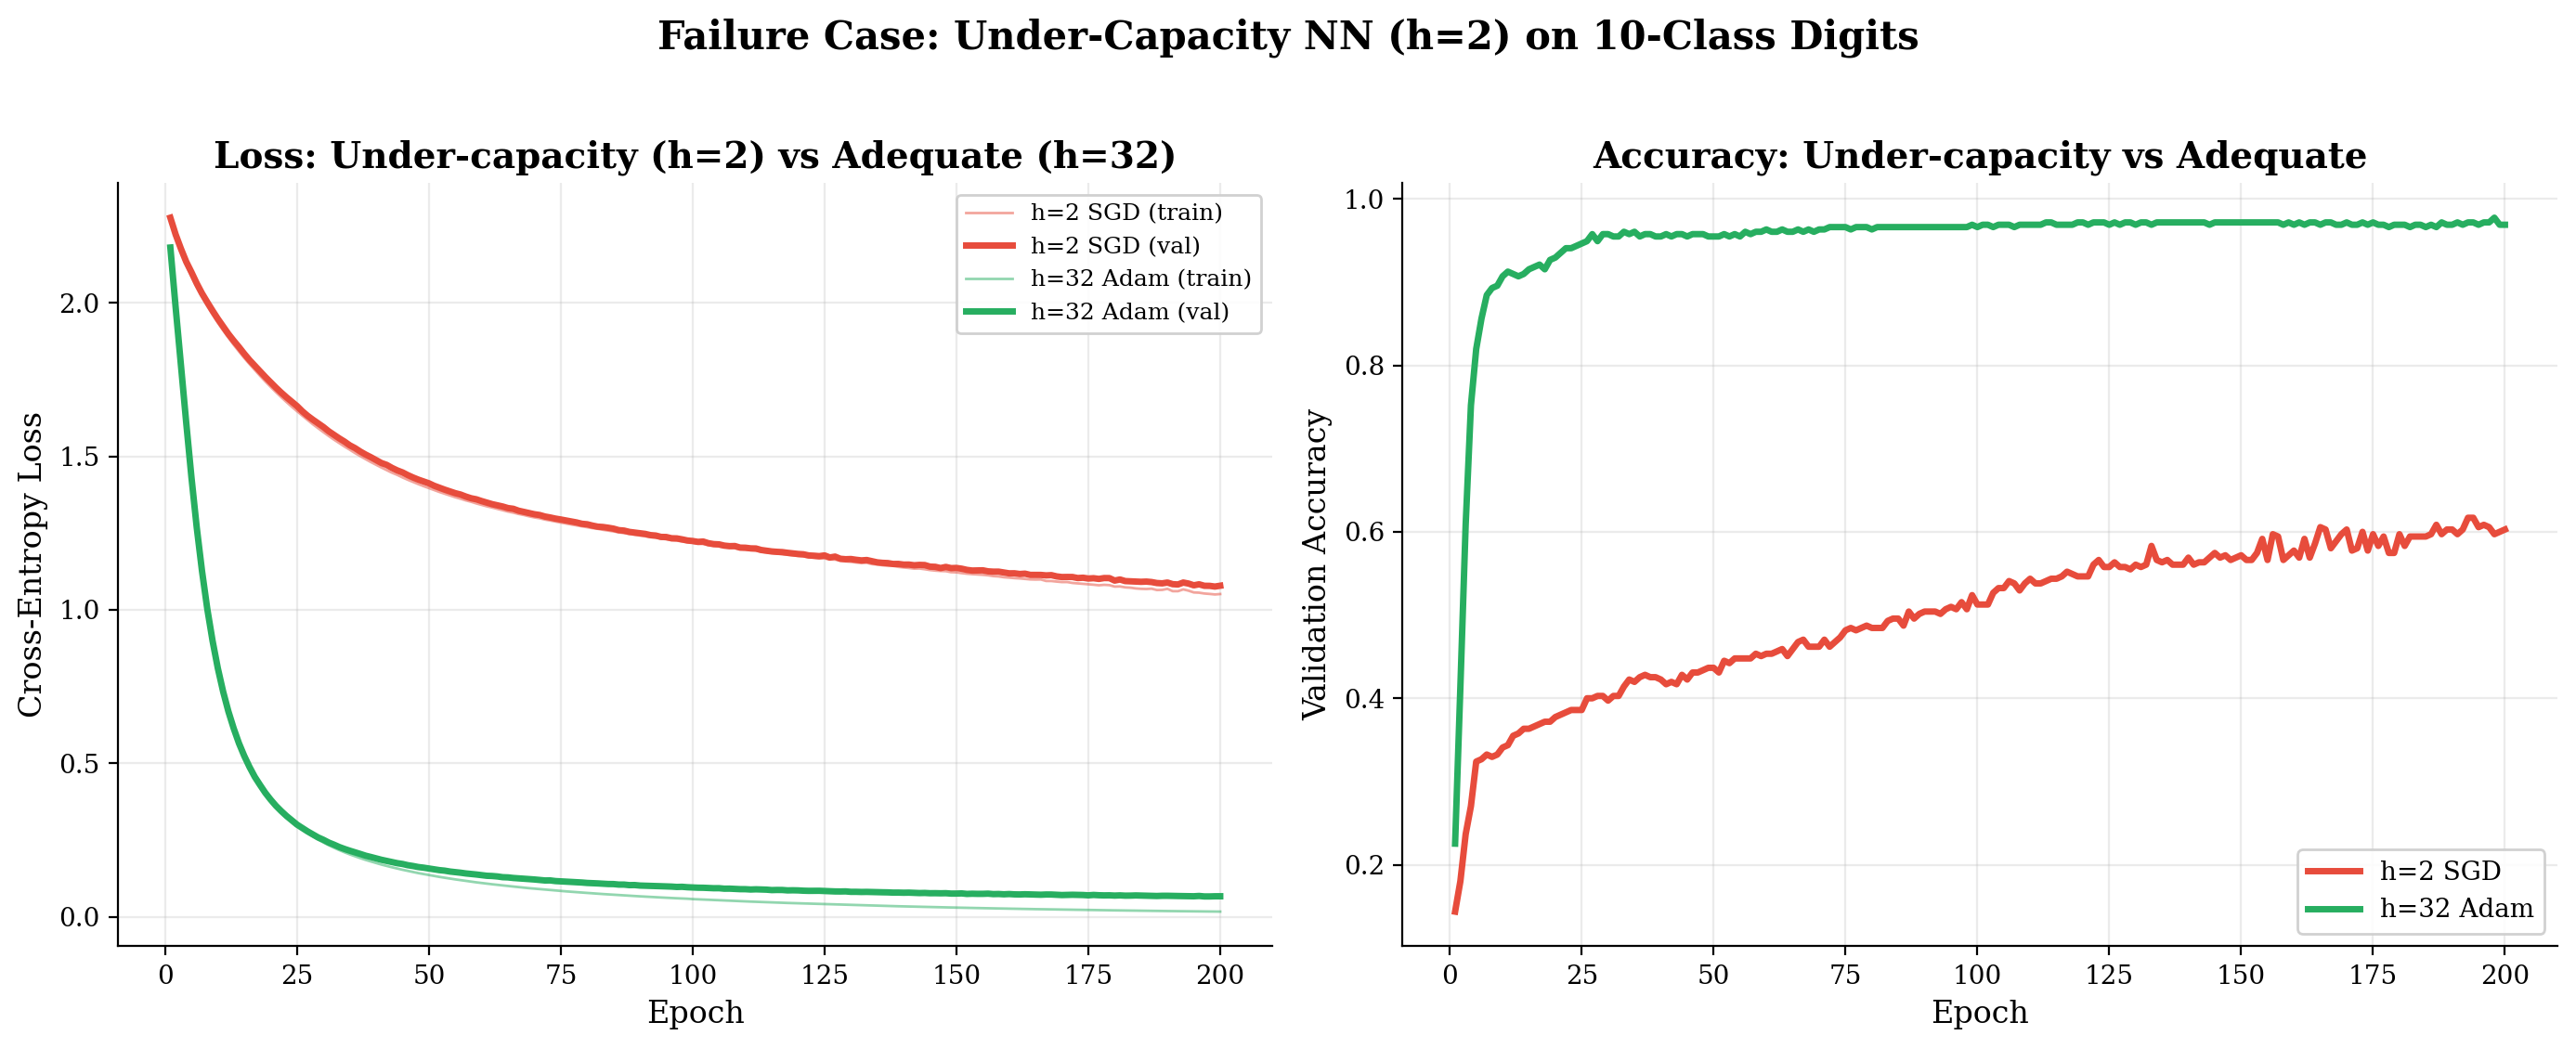
\includegraphics[width=\textwidth]{../figures/failure_analysis.png}
  \caption{Failure case.  Left: $H{=}2$ severely underfits with high residual loss.
           Right: $H{=}32$ converges to low loss.}
  \label{fig:failure}
\end{figure}

% ================================================================
\section{Advanced Track A: PCA/SVD and Input Geometry}
\label{sec:pca}
% ================================================================

To study the linear structure already present in the Digits input space, we computed the singular
value decomposition (SVD) of the mean-centred data matrix $\bX_c = \bX - \bar{\bx}^\top$.

\paragraph{Scree analysis.}
Figure~\ref{fig:pca_scree} plots the individual and cumulative explained variance ratios.  The
decay is rapid:

\begin{center}
\begin{tabular}{@{}lcccc@{}}
\toprule
Components $m$ & 5 & 10 & 20 & 40 \\
\midrule
Cumulative variance & 54.7\% & 74.1\% & 89.6\% & 98.9\% \\
\bottomrule
\end{tabular}
\end{center}

\noindent
The top 20 components already retain $89.6\%$ of total variance; the remaining
44~dimensions contribute only noise-level variance.

\paragraph{2-D projection.}
Figure~\ref{fig:pca_2d} shows the Digits data projected onto the first two principal components.
Some digit classes (e.g.\ 0 and 6) form distinct clusters, while others (e.g.\ 3, 5, 8) overlap
substantially---indicating that two dimensions are insufficient for full separation but reveal
meaningful coarse structure.

\paragraph{Classification at reduced dimensions.}
Table~\ref{tab:pca} reports Softmax Regression validation accuracy when the input is
PCA-compressed to $m$ dimensions:

\begin{table}[H]
\centering
\caption{Softmax Regression accuracy on PCA-reduced Digits inputs.}
\label{tab:pca}
\begin{tabular}{@{}lcccc@{}}
\toprule
$m$ & 10 & 20 & 40 & 64 (full) \\
\midrule
Val.\ Accuracy & 92.68\% & 94.08\% & 94.93\% & 95.49\% \\
Val.\ CE Loss  & 0.2874  & 0.2292  & 0.2133  & 0.2109  \\
\bottomrule
\end{tabular}
\end{table}

At $m{=}20$ (capturing $89.6\%$ of variance), Softmax Regression still achieves $94.08\%$
accuracy---only $1.4$ percentage points below the full-dimensional result.  This reveals that
\textbf{the Digits input space contains substantial linear structure}: a linear model can classify
well even after discarding $68.75\%$ of the original dimensions.  In contrast, the modest but
consistent 2.5-point advantage of the neural network ($H{=}32$) over Softmax on the full
64-dimensional input suggests that the nonlinear features captured by the hidden layer exploit
\emph{residual} structure that PCA---being a purely linear projection---cannot recover.

\begin{figure}[H]
  \centering
  \begin{subfigure}[b]{0.48\textwidth}
    \centering
    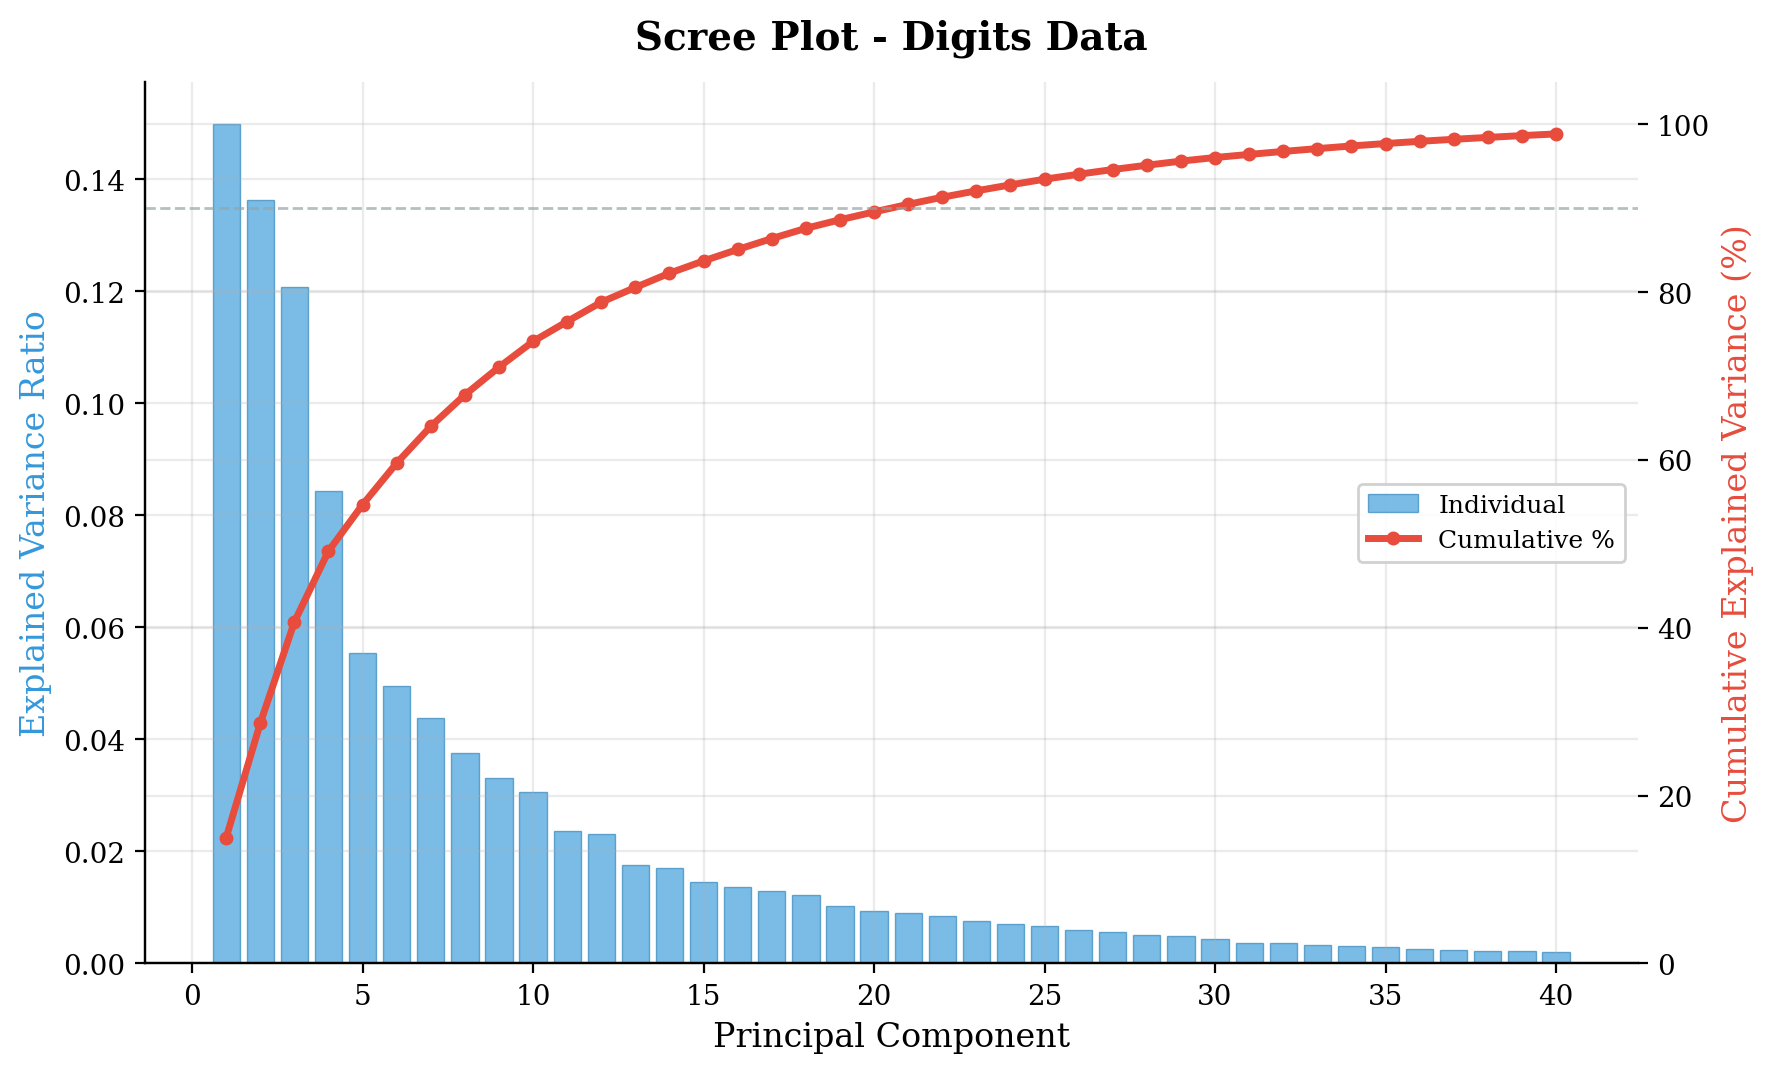
\includegraphics[width=\textwidth]{../figures/pca_scree_digits.png}
    \caption{Scree plot and cumulative variance.}
    \label{fig:pca_scree}
  \end{subfigure}\hfill
  \begin{subfigure}[b]{0.48\textwidth}
    \centering
    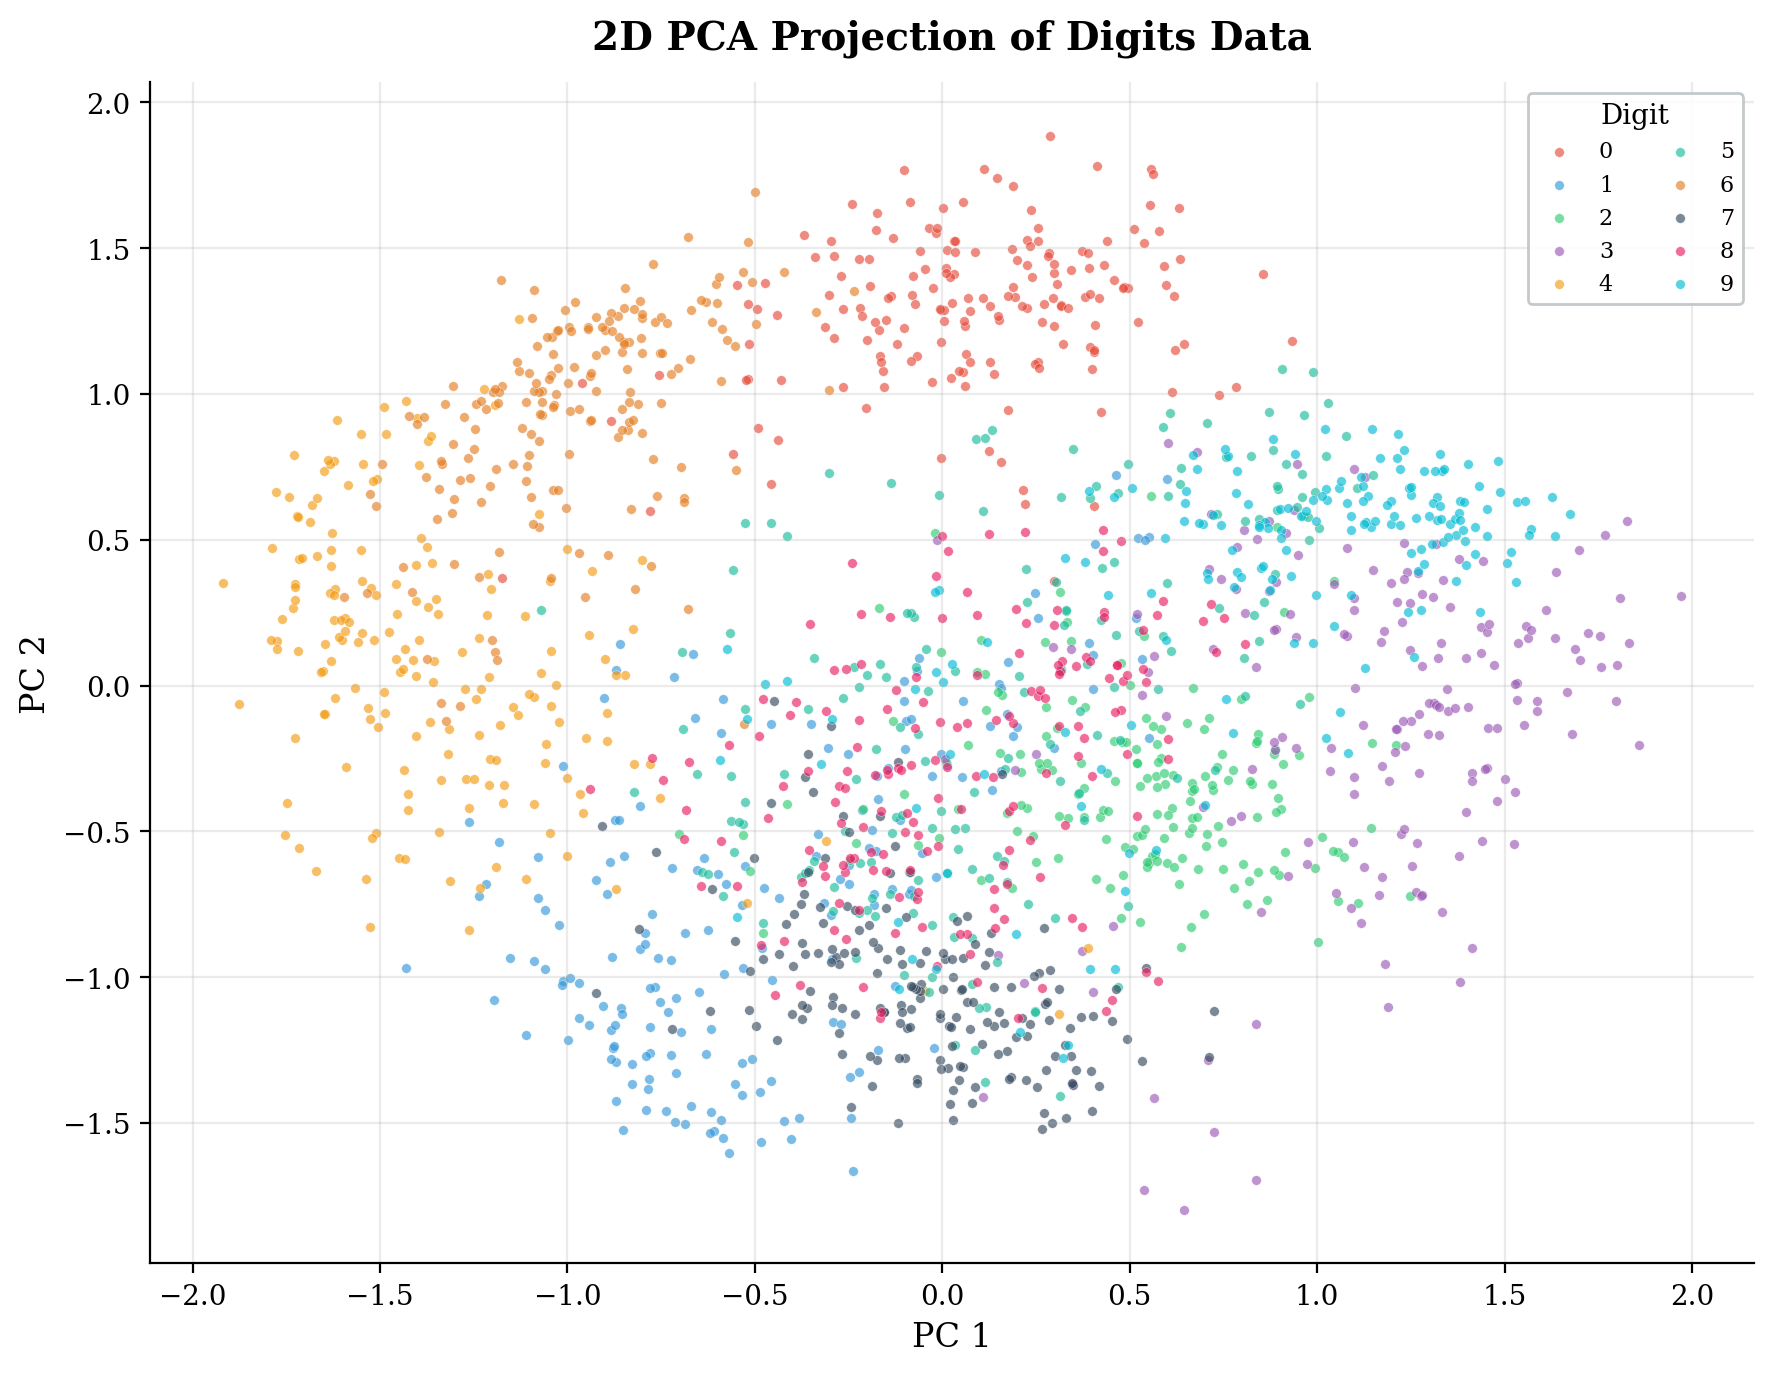
\includegraphics[width=\textwidth]{../figures/pca_2d_digits.png}
    \caption{2-D PCA projection of Digits classes.}
    \label{fig:pca_2d}
  \end{subfigure}
  \caption{Track A: PCA/SVD analysis of the Digits dataset.}
  \label{fig:pca}
\end{figure}

% ================================================================
\section{Discussion: Interpretive Analysis}
\label{sec:discussion}
% ================================================================

We now answer the five core interpretive questions required by the capstone, drawing exclusively
on the evidence produced above.

\begin{enumerate}[leftmargin=2em,itemsep=0.5em]

\item \textbf{When is the linear model geometrically sufficient, and when is it not?}

The linear model is sufficient whenever the Bayes-optimal decision boundary is a hyperplane (or
close to one).  This is rigorously the case for the Gaussian task (Section~\ref{sec:geometry})
and approximately true for the Digits benchmark, where Softmax Regression already reaches
$93.26\%$ accuracy.  The PCA experiment (Section~\ref{sec:pca}) reinforces this: even after
aggressive dimensionality reduction, linear classification remains strong, because the dominant
variance directions align with class-discriminative directions.

The linear model is \emph{insufficient} when the class-conditional distributions create decision
boundaries that must curve.  On the Moons task, no affine function can separate the two arcs, and
Softmax Regression produces a qualitatively wrong boundary (Figure~\ref{fig:comparison_moons}).

\item \textbf{What representational change does the hidden layer provide?}

The hidden layer applies the map $\bh = \tanh(\bW_1\bx + \bb_1)$, which is a learned nonlinear
coordinate change from $\R^d$ to $\R^H$.  In the new coordinates, previously entangled classes
may become linearly separable.  On the Moons task, this is visible as the transformation from
curved, interleaving arcs in $\R^2$ to distinct clusters in $\R^{32}$ that the output layer can
separate with a hyperplane.  On Digits, the hidden layer extracts nonlinear feature combinations
(e.g.\ stroke curvatures, junctions) that a linear projection cannot capture, accounting for the
${\sim}2.5$-point accuracy gain.

\item \textbf{When does additional model complexity fail to justify itself?}

Complexity fails to justify itself when the linear baseline already captures the essential
decision geometry.  On the Gaussian task, the neural network does not improve accuracy over
Softmax Regression; it merely adds $H(d+K)+H+K$ unnecessary parameters.  In the PCA experiment,
Softmax Regression at $m{=}20$ achieves $94.08\%$---within $1.6$ points of the full neural
network ($95.71\%$) while using a far simpler model on a third of the original dimensions.  These
cases show that additional parameters extract negligible benefit when the task's intrinsic geometry
is already well-matched by the simpler model class.

\item \textbf{What does your failure case teach about optimisation, capacity, or generalisation?}

The $H{=}2$ bottleneck experiment (Section~\ref{sec:failure}) teaches that
\emph{representational capacity is a prerequisite that optimisation cannot substitute}.  Despite
using the same optimiser, learning rate, and epoch budget that yield $95.71\%$ with $H{=}32$, the
$H{=}2$ model stalls at $58.97\%$.  The bottleneck is not in the loss landscape's ability to be
traversed, but in the function class's ability to represent the needed mapping.  Two hidden
dimensions cannot support 10~linearly separable clusters, so even the global minimum of the
$H{=}2$ loss surface corresponds to a poor classifier.  This is a clear instance of
\emph{underfitting due to model capacity constraints}, not of poor generalisation or bad
optimisation.

\item \textbf{What do repeated-seed statistics add beyond a single run?}

A single training run's outcome depends on the random initialisation of~$\bW_1,\bW_2$ and the
mini-batch permutation order.  A ``lucky'' seed may start near a good local minimum and yield
high accuracy; an ``unlucky'' seed may not.  By running five seeds and reporting
$\bar{x}\pm t_{0.025,4}\cdot s/\!\sqrt{5}$, we bound the \emph{expected} performance under
typical initialisation rather than reporting a cherry-picked optimistic result.  Concretely,
both models show tight intervals (Softmax: $\pm 0.73\%$; NN: $\pm 0.91\%$), confirming that
the ${\sim}2.5$-point gap is robust and not an artefact of one favourable seed.

\end{enumerate}

% ================================================================
\section{Limitations}
% ================================================================

Several boundaries constrain the conclusions of this study:

\begin{enumerate}[leftmargin=2em,itemsep=0.3em]
  \item \textbf{Architectural scope.}
        We test only a single hidden layer with $\tanh$ activations and widths up to $H{=}32$.
        Our conclusions about when nonlinearity helps do not extend to deeper networks, wider
        layers, or other activation families (e.g.\ ReLU, GELU).

  \item \textbf{Dataset scale and diversity.}
        The Digits benchmark has $d{=}64$, $K{=}10$, and ${\sim}1\,800$ total samples.  Results
        may not generalise to high-resolution images, natural-language data, or tasks with
        hundreds of classes.

  \item \textbf{Optimiser exploration.}
        The three optimisers are tested with single fixed hyperparameter settings.  We cannot
        claim that SGD is fundamentally inferior to Adam; a different learning rate or schedule
        could change the ranking.

  \item \textbf{Regularisation.}
        We use only $L_2$ regularisation ($\lambda{=}10^{-4}$).  Techniques such as dropout,
        batch normalisation, learning-rate warm-up, or gradient clipping might change the
        relative advantage of the neural network on Digits.

  \item \textbf{Repeated-seed sample size.}
        Five seeds provide a coarse estimate of variability.  The $t$-based confidence intervals
        assume approximate normality; with only five observations, this assumption is
        difficult to verify rigorously.

  \item \textbf{Synthetic task simplicity.}
        The Gaussian and Moons datasets are 2-D with 400~points and noise-free class labels.
        They illustrate geometric principles clearly but do not represent the ambiguity and noise
        of real-world classification tasks.

  \item \textbf{Generalisation claims.}
        All test-set evaluations are conducted on a single fixed split.  A more robust
        assessment would use cross-validation or multiple independent splits, which was outside
        the scope of this project.
\end{enumerate}

In summary, our findings reliably characterise the specific comparison between Softmax Regression
and a minimal one-hidden-layer network on the three provided tasks.  They should not be
over-generalised to deeper architectures, larger datasets, or more sophisticated training
pipelines.

% ================================================================
\newpage
\section*{References}
% ================================================================
\begin{enumerate}[label={[\arabic*]},leftmargin=2em,itemsep=0.2em]
  \item Goodfellow,~I., Bengio,~Y., \& Courville,~A.\ (2016). \textit{Deep Learning}. MIT
        Press.
  \item Deisenroth,~M.\,P., Faisal,~A.\,A., \& Ong,~C.\,S.\ (2020). \textit{Mathematics for
        Machine Learning}. Cambridge University Press.
  \item Murphy,~K.\,P.\ (2022). \textit{Probabilistic Machine Learning: An Introduction}. MIT
        Press.
  \item Ng,~A.\ \& Katanforoosh,~K. \textit{CS229 Lecture Notes: Deep Learning}. Stanford
        University.
  \item Stanford CS231n staff. \textit{Neural Networks Part 1: Setting up the Architecture}.
        \url{https://cs231n.github.io/neural-networks-1/}
  \item Stanford CS231n staff. \textit{Optimization Part 2: Backpropagation, Intuitions}.
        \url{https://cs231n.github.io/optimization-2/}
  \item ETH Zurich Learning and Adaptive Systems Group. \textit{Introduction to Machine Learning
        Course Notes}. \url{https://las.inf.ethz.ch/teaching/introml-s24}
  \item Math4AI Program Handout: \textit{Math4AI Capstone: From Linear Scores to a Single Hidden
        Layer}.
\end{enumerate}

\end{document}
